%“
\documentclass[12pt]{article}
\usepackage[utf8]{inputenc}
\usepackage{chemfig}
\usepackage[version=4]{mhchem}
\usepackage{amsfonts}
\usepackage{amsmath}
\usepackage{amssymb}
\usepackage{geometry}
\usepackage{mathabx}
\usepackage{relsize}
\usepackage{graphics}
\usepackage[colorlinks = true,
            linkcolor = blue,
            urlcolor  = blue,
            citecolor = blue,
            anchorcolor = blue]{hyperref}
%\usepackage{indentfirst}
\usepackage{tikz}
\usepackage{listings}
\usepackage{sidecap}
\usepackage{comment}
\geometry{
 a4paper,
 total={6.5in,0in},
 left= 15mm,
 top= 15mm,
 bottom=15mm,
 right = 15mm
 }
\usepackage[sorting=none]{biblatex}
\addbibresource{References.bib}
\title{\vspace{-2cm}COVID Spread Outdoors: Scientific Literature Review}
\author{Marcos Perez}
\date{January 15, 2022-}
\begin{document}
\maketitle
\begin{comment}
Copy paste and fill in the below template to add a new entry
\item \href{}{}
\begin{lstlisting}[breaklines]
\end{lstlisting}
\end{comment}
\section{Disclaimers}
\textbf{\textit{Please always only defer to public health and medical professionals for medical advice}. }\par
 I am not a professional COVID researcher, nor am I a biologist, nor have I earned any medical degrees, nor a PhD (yet). I am just a Caltech undergraduate who has presented at several research conferences in astrophysics, planetary science, geophysics, geology, and photonics. I am well aware that this is not my field of expertise, which is why I carefully review existing research and consult biologists rather than conducting any original research of my own.\\
\section{Introduction}
For the sake of time and energy, this will mostly consist of quotes, references, and some limited synthesis and conclusions. Although the risk of spreading COVID is reduced by being outdoors instead of being indoors, the risk is not completely eliminated. Here, I will do my best to review relevant recent, peer reviewed, scientific research conducted by professionals. Specifically, I am focused on research that quantifies the risk of spreading of COVID outside, what factors affect said risk, and how they can be mitigated. 
\section{Empirical Evidence}
“A survey of the existing literature indicates that this
increase in risk with a physical activity level associated with various
common scenarios is under-appreciated."\cite{noauthor_mathematical_nodate}
\section{Simulations}
\subsection{\textit{A mathematical framework for estimating
risk of airborne transmission of COVID-19
with application to face mask use and
social distancing} \cite{noauthor_mathematical_nodate}}
“Furthermore, even in outdoor settings, the presence
of high human density (such as at sporting events, social gatherings,
and so on) could introduce significant anthropogenic effects on the
dispersion and transport of respiratory aerosols."
“Outdoors, these are dispersed upward into the
atmosphere, and therefore far-field aerosol transmission is
unlikely outdoors given greater ventilation."\\
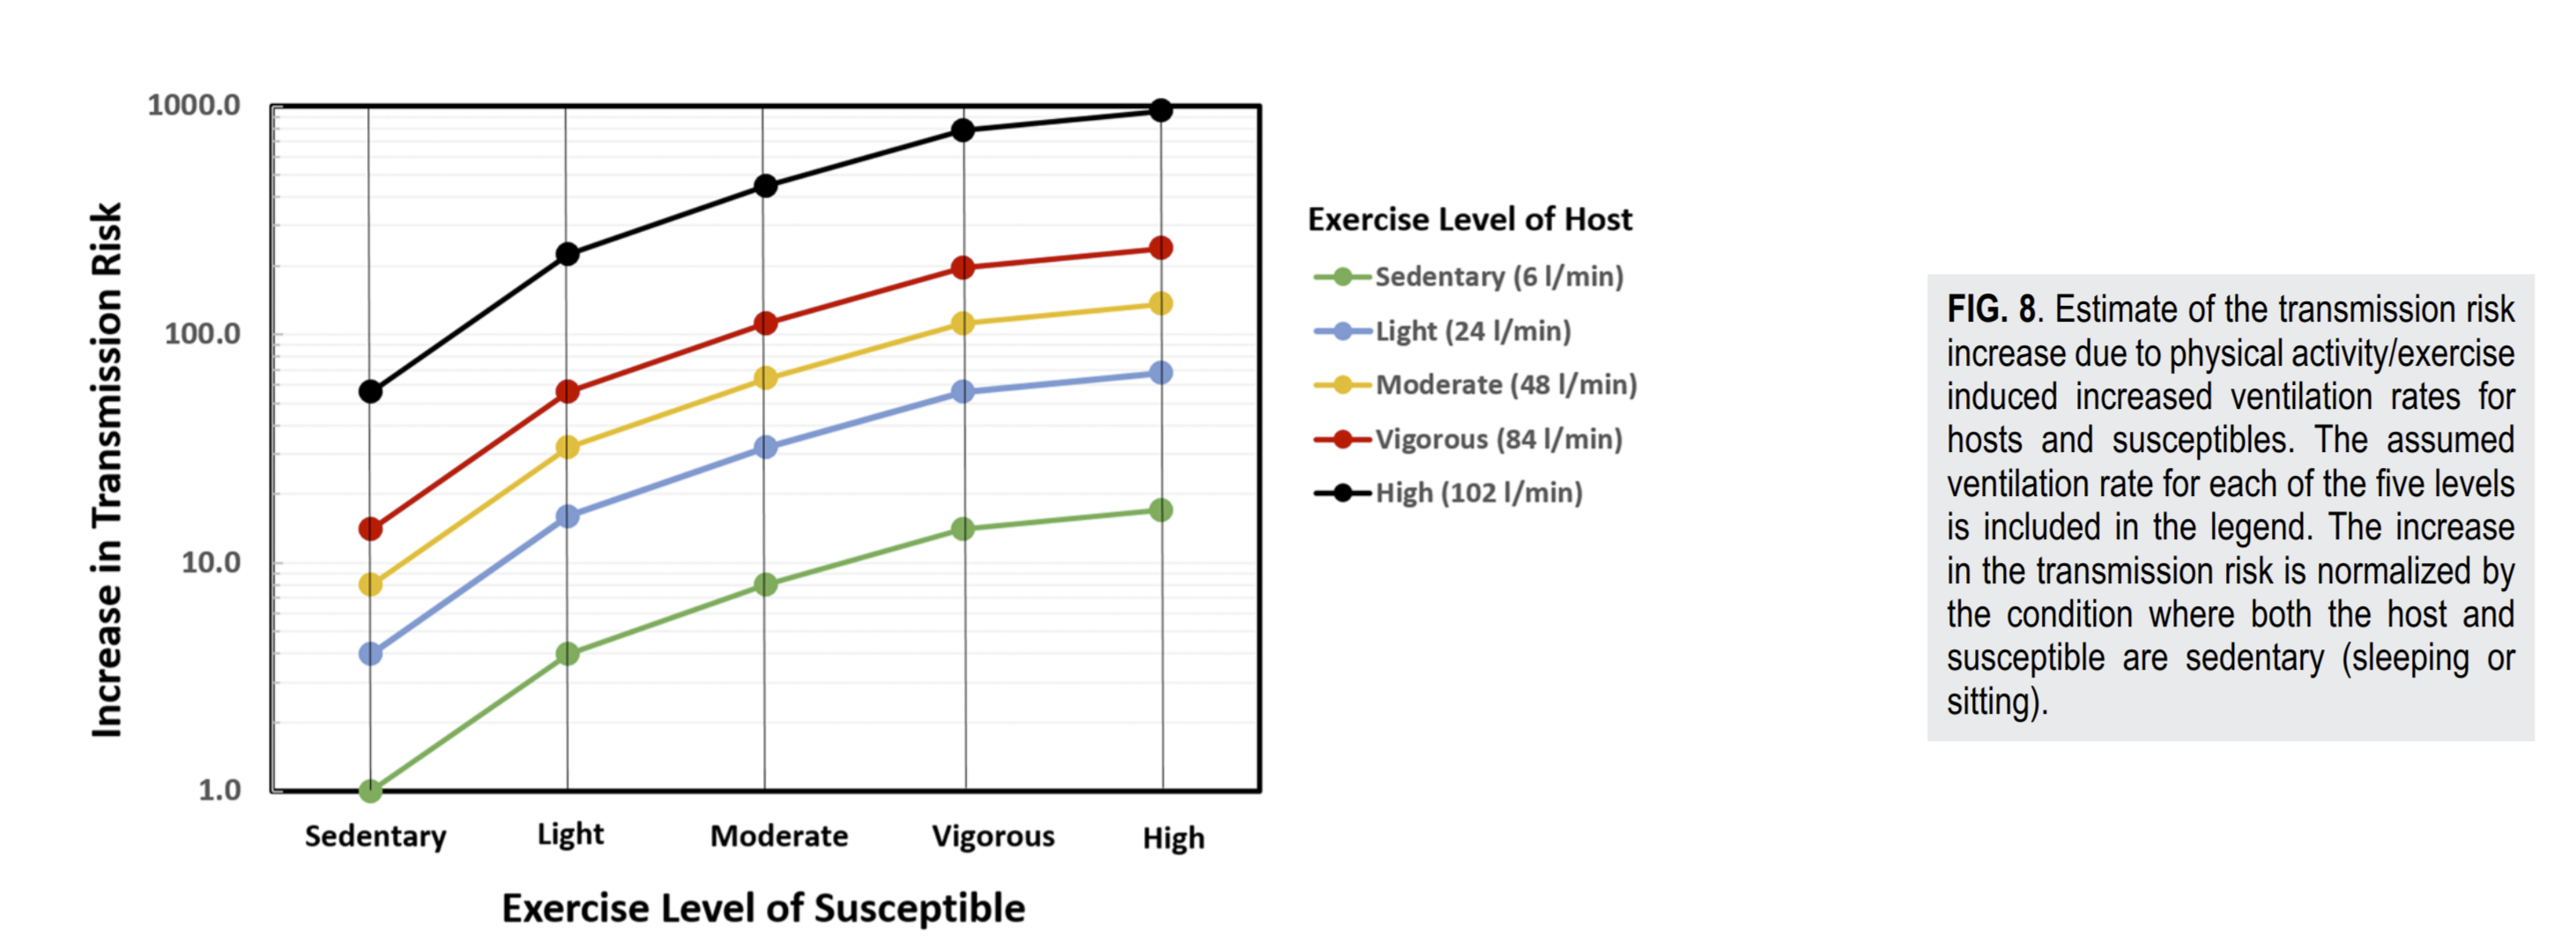
\includegraphics[scale=.6]{Images/Figure Screenshots/Estimate of the transmission risk.PNG}\\
“In a facility such as a gym or, for instance,
a basketball practice, where exercise intensity levels could be in the
'vigorous' range, the transmission risk could be nearly 200 times
higher due to increased exhalation and inhalation rates of the individuals involved."\\
“The approximately inverse relationship of the transmission risk and spatial distance from physical distancing is one example of the important insights that can be generated by the model." Thus, the referenced model for COVID transmission through the air agrees with the current consensus that physical distance is an effective form of social distancing. However, it is important to acknowledge a seldom recognized finding, that airborne COVID transmission is also strongly dependent on exercise and respiration rate.\cite{noauthor_mathematical_nodate}
\section{Conclusions and Synthesis}
\subsection{\href{https://www.zotero.org/groups/4564641/marcos\_perez\_covid\_spread\_outdoors/library}{Link to Zotero Folder}}
\begin{verbatim}
https://www.zotero.org/groups/4564641/marcos_perez_covid_spread_outdoors/library
\end{verbatim}


\printbibliography[title = \Large \textbf{References} \Large ]


\end{document}
 